\documentclass[12pt]{article}
\usepackage[utf8]{inputenc}
\usepackage{amsmath}
\usepackage{graphicx}
\usepackage{appendix}
\usepackage{listings} % for source code inserts
\title{CS 470 Spring 2011 \\
     Project 4}
\author{Colby Blair}
\date{Due May 10th, 2011}
\begin{document}
\maketitle

\begin{abstract}
There are many different approaches to implementing Artificially Intelligent agents. One approach is to use
a symbolic approach. This report will use a logic-based area of the symbolic approach. This approach does
not try to simulate the thought process of humans, but instead tries to find the basis for logical decision
making. This seems to suggest that the Turing Test isn't the best measure for intelligence, as humans 
are imperfect and often act irrational.

This report uses Prolog to implement the logic-based symbolic family tree. This approach uses a knowledge 
base that the logic agent consults. Specific relationships are defined, and more general rules are made as
well. This is a quick process, but seems to lack a core AI element (like learning) to be truely intelligent. It is,
however, much quicker, and much more logical, than other methods.
\end{abstract}

\thispagestyle{empty}

\pagebreak

\thispagestyle{empty}
\tableofcontents
\listoffigures

\pagebreak

\setcounter{page}{1}



\section{Introduction}
For this report, Prolog is used to create a family tree. For a logic based approach, Prolog is a good language. It doesn't do a lot of other things that other languages do, but it does relationships in the form of a knowledge base very well. For each possible input, there are possible outputs, much like other AI methods. If a query is 
defined in the knowledge base, the query is acknowledges with a success. Otherwise, it is a failure, which may just mean that the knowledge base is not complete.

All the rules in the knowledge base are tried until one succeeds. This equivaltes to Conjunctive Normal Form 
(CNF) statements. 

\begin{figure}[h]
        \begin{center}
		$(A \vee B) \wedge (C \vee D) \wedge ...$
                	\caption{A CNF Statement}
                	\label{cnf_ex}
        \end{center}
\end{figure}

For this report, we will consider the following family trees:
\begin{figure}[!h]
        \begin{center}
                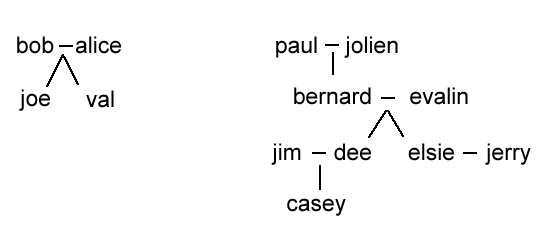
\includegraphics[width=90mm]{images/fam_tree.png}
                \caption{Family Tree}
                \label{fam_tree}
        \end{center}
\end{figure}



%  A description of the general syntax of your knowledge base works. What is the general form of the rules, examples of rules, etc.
\section{Example Knowledge Base Syntax}
There was many ways to defined relationships for the family tree. The way this report chooses to define relationships between two specific people is mostly by common parents. Most of the family tree is 
constructed this way. Being married without children, and being male or female, are the only other specific 
definition needed for each person. The full knowledge base is listed in Appendice \ref{sec:appendice a}.

\begin{figure}[h]
 \begin{lstlisting}
	parent(jim,casey).
	parent(dee,casey).

	man(jim).
	man(casey).
	woman(dee).
 \end{lstlisting}
\caption{Some specific definitions}
\label{spec}
\end{figure}

The tree is then built with this concept. Rules that do not define specific people, but relationships between 
variables, then use this parent-child structure. 

\begin{figure}[h]
 \begin{lstlisting}
	child(X,Y):- parent(Y,X).
	sibling(X,Y):- parent(Z,X),parent(Z,Y).
 \end{lstlisting}
\caption{Some definitions that use specific parent definitions}
\label{child}
\end{figure}

Consider the sibling rule in Figure \ref{child}. Prolog uses goal-based evaluation here to try every person who 
is a parent, assigns them to the 'Z' variable, and sees if some Z is a parent for both X and Y. This is an 
extremely powerful feature of Prolog, and simplifies the code. Anywhere in this knowledge base, 'Z' is used as
the search variable for conditions.



% A results section that shows sample queries and results. Include a mixture of simple queries (who is Sam's father?) and complex queries (who are all of the sisters in the knowledge base?). If there are any queries it does not answer satisfactory include examples of those.
\section{Results}
The results for searches are nice and quick:
\begin{figure}[!h]
 \begin{lstlisting}
| ?- uncle(jerry,casey).  
true ? 
yes
 \end{lstlisting}
\caption{Uncle query}
\label{q1}
\end{figure}

Even for some of the more intense questions:
\begin{figure}[!h]
 \begin{lstlisting}
| ?- related(jerry,casey).
true ? 
yes
 \end{lstlisting}
\caption{Related query}
\label{q2}
\end{figure}

\pagebreak

\begin{figure}[!h]
 \begin{lstlisting}
| ?- ancestor(paul,casey).
true ? 
yes
 \end{lstlisting}
\caption{Ancestor query}
\label{q3}
\end{figure}

Simple queries work fine too:
\begin{figure}[!h]
 \begin{lstlisting}
| ?- sister(dee,elsie). 
true ? 
yes
 \end{lstlisting}
\caption{Sisters query}
\label{q4}
\end{figure}

But the relationship issues with sibling and married are still avoided:
\begin{figure}[!h]
 \begin{lstlisting}
| ?- married(jim,dee). 
yes
| ?- married(jerry,elsie).
(1 ms) yes
| ?- married(dee,elsie).  
no
 \end{lstlisting}
\caption{Married and sibling query}
\label{q5}
\end{figure}



% A discussion section that discusses the strengths and weaknesses of your knowledge base. Are their questions it should be able to answer, but can't? Is it easy to add new rules? Is it easy to formulate general queries? Etc.
\section{Discussion}
This knowledge base choose parents as the root way to define most relationships. This had pros and cons.
There was a little more complexity with married people, because you could not define them as having 
common parents, even though they would be parent-in-laws. This would be too close to the sibling 
definition. The result was to associate them by common children, and only define real parents in the scheme.

Another con to this knowledge base is that it makes very traditional assumptions on families. If one had 
common children with another, they would be married. Although sexes aren't checked here, they are checked
under aunt and uncle definitions. 

It is very easy to add new rules to the knowledge base. So much so, that almost every rule is based off the 
parent, man, or woman rules, or off other rules that are. The special cases are kept to a minumum. General queries always take the form of 'role(X,Y)', or 'X is the role of Y'. 

Overall, Prolog is extremely powerful at this niche in compter science and AI. So much so, that it would be a
great tool to keep in the toolbox for future projects. It defines relationships very quickly, something that can
become long winded in a lower level language. It isn't as cryptic as Lisp, and has some real power with 
goal-oriented evaluation.



\section{Full Knowlede Base Definition Explanations}
\subsection{parent}
Like mentioned before, parents are one of the few definitions that use names only:
\begin{figure}[!h]
 \begin{lstlisting}
	parent(jim,casey).
	parent(dee,casey).
 \end{lstlisting}
\caption{Parent definition}
\label{spec}
\end{figure}

\pagebreak

\subsection{gender}
Simple enough:
\begin{figure}[!h]
 \begin{lstlisting}
	man(jim).
	man(casey).
	woman(dee).
 \end{lstlisting}
\caption{gender definition}
\label{spec}
\end{figure}


\subsection{child}
The reverse of parent. You are a child of someone if they are a parent of you:
\begin{figure}[!h]
 \begin{lstlisting}
	child(X,Y):- parent(Y,X).
 \end{lstlisting}
\caption{child definition}
\label{spec}
\end{figure}


\subsection{mother}
You are a mother of someone if you are a parent and a woman:
\begin{figure}[!h]
 \begin{lstlisting}
	mother(X,Y)   :- parent(X,Y),woman(X).
 \end{lstlisting}
\caption{mother definition}
\label{spec}
\end{figure}


\subsection{father}
You are a father of someone if you are a parent and a man:
\begin{figure}[!h]
 \begin{lstlisting}
	father(X,Y)   :- parent(X,Y),man(X).
 \end{lstlisting}
\caption{father definition}
\label{spec}
\end{figure}


\subsection{sister}
You are a sister of someone if you are a sibling and a woman:
\begin{figure}[!h]
 \begin{lstlisting}
	sister(X,Y)   :- sibling(X,Y),woman(X).
 \end{lstlisting}
\caption{sister definition}
\label{spec}
\end{figure}


\subsection{brother}
You area a brother os someone if you are a sibling and a man:
\begin{figure}[!h]
 \begin{lstlisting}
	brother(X,Y)  :- sibling(X,Y),man(X).
 \end{lstlisting}
\caption{brother definition}
\label{spec}
\end{figure}


\subsection{sibling}
You are a sibling of someone if you have common parents:
\begin{figure}[!h]
 \begin{lstlisting}
	sibling(X,Y):- parent(Z,X),parent(Z,Y).
 \end{lstlisting}
\caption{sibling definition}
\label{spec}
\end{figure}


\subsection{aunt}
You (X) are an aunt of someone if you are either a). a sister of some Z, and that Z is a parent of Y, or 
b). married to some Z, and that Z is an uncle to Y.
\begin{figure}[!h]
 \begin{lstlisting}
	aunt(X,Y)     :- 	(sister(X,Z),parent(Z,Y));
				(married(X,Z),uncle(Z,Y)).
 \end{lstlisting}
\caption{aunt definition}
\label{spec}
\end{figure}

\pagebreak

\subsection{uncle}
You (X) are a uncle of someone if a). you are a brothr of some Z, and that Z is a parent of Y, or 
b). you are married to some Z, and they are an aunt to some y.
\begin{figure}[!h]
 \begin{lstlisting}
	uncle(X,Y)    :- 	(brother(X,Z),parent(Z,Y)); 
				(married(X,Z),aunt(Z,Y)).
 \end{lstlisting}
\caption{uncle definition}
\label{spec}
\end{figure}


\subsection{related}
This report tried to use ancestor and decendent to implement 'related', but got stack overflows. This was
probably an issue with infinite recursion. The solution was to use rules like ancestor and decendent. If you
(X) are related to Y, then you are a parent, child, or married to someone that is a parent, child, or married to,
someone who... through recursion, is eventual a parent, child, or married to some relation to you.
\begin{figure}[!h]
 \begin{lstlisting}
	related(X,Y)  :- parent(X,Y).
	related(X,Y)  :- parent(X,Z),related(Z,Y).
	related(X,Y)  :- child(X,Y).
	related(X,Y)  :- child(X,Z),related(Z,Y).
	related(X,Y)  :- married(X,Y).
	related(X,Y)  :- married(X,Z),related(Z,Y).
 \end{lstlisting}
\caption{related definition}
\label{spec}
\end{figure}


\subsection{decendent}
You (X) are a decendent if you are a child of someone who is a child of someone... recursively, until someone who is a child of the ancestor (Y).
\begin{figure}[!h]
 \begin{lstlisting}
	decendent(X,Y):- child(X,Y).
	decendent(X,Y):- child(X,Z),decendent(Z,Y).
 \end{lstlisting}
\caption{decendent definition}
\label{spec}
\end{figure}


\subsection{ancestor}
You (X) are an ancestor of someone if you are a parent to someone who is a parent... recursively, until 
someone who is a parent of a child (Y).
\begin{figure}[!h]
 \begin{lstlisting}
	ancestor(X,Y) :- parent(X,Y).
	ancestor(X,Y) :- parent(X,Z),ancestor(Z,Y).
 \end{lstlisting}
\caption{ancestor definition}
\label{spec}
\end{figure}

 

\pagebreak

% An appendix containing the full knowledge base.
\appendix
\appendixpage
\addappheadtotoc

\section{The full Knowledge Base}
\label{sec:appendice a}

 \begin{lstlisting}
%(X,Y) - X is a <> of Y

%specific definitions
parent(bob,joe).
parent(alice,joe).
parent(bob,val).
parent(alice,val).
parent(paul,bernard).
parent(jolien,bernard).
parent(bernard,dee).
parent(evalin,dee).
parent(bernard,elsie).
parent(evalin,elsie).
parent(jim,casey).
parent(dee,casey).

%specific definitions
man(joe).
man(bob).
man(jerry).
man(jim).
man(casey).
man(paul).
woman(val).
woman(alice).
woman(elsie).
woman(dee).
woman(jolien).

%non-sex specific statements
child(X,Y):- parent(Y,X).
sibling(X,Y):- parent(Z,X),parent(Z,Y).
married(X,Y)  :- parent(X,Z),parent(Y,Z). 	%have common children
	married(jerry,elsie). 			%don't have children

%sex specific statements
father(X,Y)   :- parent(X,Y),man(X).
mother(X,Y)   :- parent(X,Y),woman(X).
sister(X,Y)   :- sibling(X,Y),woman(X).
brother(X,Y)  :- sibling(X,Y),man(X).
aunt(X,Y)     :- (sister(X,Z),parent(Z,Y));(married(X,Z),uncle(Z,Y)).
uncle(X,Y)    :- (brother(X,Z),parent(Z,Y));(married(X,Z),aunt(Z,Y)).

%others
ancestor(X,Y) :- parent(X,Y).
ancestor(X,Y) :- parent(X,Z),ancestor(Z,Y).
decendent(X,Y):- child(X,Y).
decendent(X,Y):- child(X,Z),decendent(Z,Y).
related(X,Y)  :- parent(X,Y).
related(X,Y)  :- parent(X,Z),related(Z,Y).
related(X,Y)  :- child(X,Y).
related(X,Y)  :- child(X,Z),related(Z,Y).
related(X,Y)  :- married(X,Y).
related(X,Y)  :- married(X,Z),related(Z,Y).

\end{lstlisting}



\end{document}
